\documentclass[10pt,a4paper]{article}
\usepackage[latin1]{inputenc}
\usepackage[T1]{fontenc}
\usepackage{amsmath}
\usepackage{amsfonts}
\usepackage{amssymb}
\usepackage{graphicx}
\usepackage{comment}
\usepackage{natbib}

\bibliographystyle{evolution.bst}

\newcommand{\norm}[1]{\left\lVert#1\right\rVert}
\newcommand{\normsq}[1]{\left\lVert#1\right\rVert^2}


\newcommand{\MX}{\mathbf{X}} %uncentered data
\newcommand{\MC}{\mathbf{C}} %centering
\newcommand{\MY}{\mathbf{Y}} %centered data
\newcommand{\MF}{\mathbf{F}_2} %F2-distance matrix
\newcommand{\MFT}{\mathbf{F}_3} %F3-distance matrix
\newcommand{\MP}{\mathbf{P}} % PCs
\newcommand{\ML}{\mathbf{L}} % loadings
\newcommand{\MK}{\mathbf{K}} % Kernel
\newcommand{\MSINGULAR}{\mathbf{\Sigma}} % Singular values matrix
\newcommand{\MEIGEN}{\mathbf{\Lambda}} % Eigenvalue matrix


\newcommand{\MEAN}{\boldsymbol{\mu}} % Kernel
\begin{document}
\section{A geometric interpretation of $F$-statistics}
$F$-statistics have been primarily motivated by trees and admixture graphs \citep{patterson2012, peter2016}, but the calculations hold up in a much wider data space. In particular,  \cite{oteo-garcia2021} provides a thorough introduction to interpreting $F$-statistics in the \emph{data space} $\mathbb{R}^k$. Their work builds much of the foundation of this discussion, by demonstrating analogies to classical geometry. A brief summary of their key results: A population's allele frequencies can be thought of as vector in $\mathbb{R}^k$. Then, $F_2(X_1, X_2) = \normsq{X_1 - X_2}$ is the squared Euclidean distance between the populations with vectors $X_1$ and $X_2$, and $F_4(X_1, X_2 ; X_3, X_4) = \langle X_1 - X_2, X_3 - X_4 \rangle$ is the inner (scalar) product between these two vectors. Here, I will mainly use the $F$-statistic notation, but use the geometric notation where convenient.

In this paper, the main focus is to use this interpretation of $F$-statistics in the context with principal component analysis (PCA), another widely used multivariate analysis tool in population genetics \citep{cavalli-sforza1994, reich2008, novembre2008, mcvean2009}. Informally, PCA is a rotation of the data such that the axis of highest variation is the first PC. The second PC th
	
\section{Relationship of PCA, $F_2$ and Outgroup-$F_3$}
	Let us assume we have some genotype data $\MX$, which contains data from $n$ on the populations on the rows, and $k$ loci on columns. Each population may be represented by a single (pseduo-)haploid, diploid individual, but in general will be an aggregation of one or many samples.
	
	To analyze this data, we might perform a PCA. A standard way of doing this is to do first center the matrix by subtracting the mean allele frequency from each column and perform an Singular Value Decomposition (SVD):
	
	\begin{equation}
	\MY = \MC\MX = \mathbf{U} \MSINGULAR \mathbf{V}^T = \MP\ML
	\end{equation}
	
	Here, $\MC = \mathbf{I} -\frac{1}{n}\mathbf{1}$ is a centering matrix and $\mathbf{I}, \mathbf{1}$ are the identity matrix and a matrix of ones, respectively. $\MP=\mathbf{U}\MSINGULAR$ is the matrix of principal components (PCs), and, $\ML=\mathbf{V}^T$ is the  matrix of loadings, respectively. Occasionally, SNPs are weighted by the square-root of their variance; for now we will assume the SNPs are unweighted, and defer discussion of weighting to a later section.
	
	
	 The principal components $\MP$ are an orthogonal matrix of size $n \times n$ that are useful for understanding population structure, the loadings are an $n \times k$ orthonormal matrix that give the contribution of each SNP along each PC, it is often useful to look for outliers that might be indicative of selection \cite[e.g]{francois2010}.
	
	Equivalently, we obtain the PCs by performing an eigendecomposition of the  covariance matrix of $\MY$, denoted as $\MK$:
	 \begin{equation}
 \MK = \MY \MY^T = \mathbf{U}\MEIGEN\mathbf{U}^T = \mathbf{U}\MSINGULAR^2\mathbf{U}^T =\MP\MP^T
	\end{equation} where $\MEIGEN$ is the diagonal matrix of eigenvalues.  In cases we are interested in the loadings, they can be obtained as 
	\begin{equation}
	\ML = \MEIGEN^{-1}\MP^T\MC\MX
	\end{equation}

	
	Let $y_{il}$ denote the genotype of the $i$-th individual at the $l$-th SNP.
	
	\begin{equation}
	y_{il} = x_{il} - \mu_l
	\end{equation}
	where $\mu_l$ is the mean genotype at the $l$-th locus.
	
	The entries of the covariance matrix $\MK$ are then
	
	\begin{equation}
	k_{ij} = \sum_l y_{il} y_{jl} = \sum_l (x_{il} - \mu_l)(x_{yl} - \mu_l) = F_3(\MEAN; X_i, X_j)
	\end{equation}
	

	It is helpful to think of $\MEAN = (\mu_1, \dots \mu_k)$ as a ``fake''-individual whose allele frequency is the sample mean of the allele frequency space, it will always lie at the origin of the PC-space.
	
	Thus, we can also think of a PCA as performing a decomposition of an Outgroup-$F_3$-matrix, where we set the output to the mean of all marker allele frequencies. This is good practice if we do not have any outgroups available. However, we often also have outgroup data; for example when studying early European variation, Africans are sometimes a suitable outgroup. In this case, it would be consequential to perform an eigendecomposition of a true outgroup $F_3$-matrix.
	

	
	
This is also a useful way to establish how we can obtain $\MP$ from $\MF$ directly: Note that the row and column means of $\MK$ are zero:
\begin{equation*}
\sum_i k_{ij}= \sum_i\sum_l (x_{il}-\mu_l)(x_{jl} - \mu_l)= \sum_l(x_{jl} - \mu_l)\left[\sum_i x_{il} -\mu_l\right] = 0 \text{.}
\end{equation*}

Since $F_2(X_1, X_2) = F_2(X_1, \mu) + F_2(X_2, \mu) - 2 F_3(\mu; X_1, X_2) \\= \normsq{X_1-\mu} + \normsq{X_2 - \mu} - 2\langle X_1 - \mu, X_2 - \mu \rangle$

(not sure if geometry notation would be easier here),

\begin{equation}
\MK = \MC\MX\MX^T\MC-\frac{1}{2} \MC \MF \MC = \MP\MP^T
\end{equation}

Thus, when we mean-center the $\MF$-matrix, we subtract the $F_2$ terms in above equations; as they are invariant with respect to the column/ row means. What remains, is directly proportional to the matrix decomposed under a standard PC. 



%In summary, a PCA and an eigendecomposition of the (negative) $\MF$-matrix will give the same results, and can be thought of as an eigendecomposition of the $\MFT$-matrix of an outgroup $F_3$-matrix with the sample mean as an outgroup.


\section{Approximating uncertainty on PCA-placement}

\section{Projection using f-stats}
Suppose we have a sample $U$ we wish to project onto an existing PCA-basis made from $\MX$, and let us assume we can compute $F_2(U, X_i)$ for all $i$. The ``best'' point i
For any particular reference sample, $F_2$ places the point on the hypercircle with equation
\begin{equation}
F_2(U, X_i) = \sum_{k=1}^{n-1} (p_{ik} - u_k)^2,
\end{equation}
where $p_{ik}$ and $u_k$ are the reference and unknown coordinate on the $k$-th component, respectively. It can be shown \cite{gower1968} that the $u_k$ can be found using
\begin{equation}
\mathbf{u} = \frac{1}{2}\MEIGEN^{-1}\MP^T\mathbf{d}
\end{equation}
where $\mathbf{d}$ is a column vector with $$d_i = F_2(X_i, \MEAN) - F_2(X_i, U)$$.

Given a fixed projection, this allows us to also propagate uncertainty on a PCA plot.

\section{$F$-stats in PCA-space}
The PCA aims to reveal the axes of major variance. The data is then ``rotated'' such that these axes can be visualized. Usually, only the first few PCs are considered. 

However, as $F_2$ is a squared Euclidean distance of allele frequencies, it is invariant to rotation and translation. Hence, neither mean-centering, which is a translation nor PCA-rotation will change $F_2$.

What this means is that we are free to calculate $F_2$ either on the uncentered data $\MX$, the centered data $\MY$ or the principal components $\MP$. Formally,

\begin{eqnarray}
F_2(X_i, X_j) &=& \sum_{l=1}^L \big( (x_{il} - \mu_l) -(x_{jl} -\mu_l)\big)^2 = F_2(Y_i, Y_j)\nonumber\\
&=& \sum_{l=1}^L \big( \sum_k L_{kl}P_{ik} - \sum_kL_{kl}P_{kj}\big)^2\nonumber\\
&=& \sum_{l=1}^L \left( \sum_k L_{kl} (P_{ik} -P_{jk}) \right)^2\nonumber\\
&=& \sum_{l=1}^L \left( \sum_k L_{kl}^2 (P_{ik} -P_{jk})^2 + 2\sum_{k\neq k'} L_{kl}L_{k'l}(P_{ik} - P_{jk'})^2 \right)\nonumber\\
&=& \sum_k \left(\sum_{l=1}^L L_{kl}^2\right) (P_{ik} -P_{jk})^2 + \sum_{k\neq k'}\left(\sum_{l=1}^L L_{kl}L_{k'l}\right) (P_{ik} - P_{jk'})^2\nonumber\\
&=& \sum_k (P_{ik} - P_{jk})^2
\end{eqnarray}


In summary, the first row shows that $F_2$ on the centered data will give the same results (as distances are invariant to translations), in the second row we apply the PC-decomposition. The third row is obtained from factoring out $L_{lk}$. Row four is obtained by multiplying out the sum inside the square term for a particular $l$. We have $k$ terms when for $\binom{k}{2}$ terms for different $k$'s.  Row five is obtained by expanding the outer sum and grouping terms by $k$.The final line is obtained by recognizing that $\ML$ is an orthonormal basis; where dot products of different vectors have lengths zero.

Note that if we estimate $F_2$, unbiased estimators are obtained by subtracting the population-heterozygosities $H_i, H_j$ from the statistic. As these are scalars, they do not change above calculation.

SHORT VERSION
\begin{align}
F_2(X_i, X_j) &=&  \sum_{l=1}^L \big( x_{il} -x_{jl}\big)^2 - H_i - H_j &&\nonumber\\ 
 &=& \sum_{l=1}^L \big( (x_{il} - \mu_l) -(x_{jl} -\mu_l)\big)^2 - H_i - H_j  &=& F_2(Y_i, Y_j) \nonumber\\
 &=& \sum_k (P_{ik} - P_{jk})^2 - H_i - H_j &=& F_2(P_i, P_j)
\end{align}
As $F_3$ and $F_4$ can be written as sums of various $F_2$-terms, analogous relations apply.

\subsection{$F$-stats in 2-dimensional PC-space}
 It is useful to consider the statistics on a PCA plot. The relationships we will discuss formally only hold in the full, $n$-dimensional PCA-space where we consider all principal components. Here, we start by discussing 2-dimensional spaces. This is useful for two reasons: for one, the geometry is simpler and we can think of circles and squares as opposed to hyperspheres and other high-dimensional geometric objects and thus help us build intuition. Second, in many applications it is argued that a 2-dimensional approximation is sufficient to explain the major components of population structure. In this case, the results here will hold under the same approximation assumptions in low-dimensional PCs; if they differ substantially from each other, it is likely that not sufficiently many PCs were considered.


\subsubsection{$F_2$ in PC-space}
The $F_2$-statistic as the squared Euclidean distance is the easiest to understand, it corresponds directly to the squared distance in PCA-space. This matches our intuition that closely related populations (which have low $F_2$) will be close to each other on a PCA-plot.

\subsubsection{$F_3$ and circles}
The $F_3$-statistic becomes more interesting; as outlines above we either think of $F_3$ as ``outgroup''-$F$-stats or as admixture $F$-stats. In the admixture case, we may ask the following question: given two source populations $X_1$, $X_2$, where would admixed populations on a PCA plot lie? From theory, we would expect it to lie between $X_1$ and $X_2$, with the exact location depending on sample sizes \cite{brisbin2012, mcvean2009}. 

Formally, we would reject admixture if $F_3$ is negative, i.e. we are looking for the space
\begin{eqnarray}
2 F_3(X_x; X_1, X_2) &=& 2\langle  X_x - X_1, X_x - X_2 \rangle \nonumber\\
      &=& \normsq{X_x - X_1} + \normsq{X_x - X_2}  - \normsq{X_1 - X_2} \nonumber\\
      &<&0
\end{eqnarray}
By the Pythagorean theorem, $F_3 = 0 $ iff $X_1, X_2$ and $X_x$ form a right-angled triangle. Hence, the region where $F_3$ is zero is the circle with diameter through $X_1$ and $X_2$. If $X_x$ lies inside this circle, the angle is obtuse and $F_3$ is negative, otherwise it will be positive. Similarly, if we fix $X_1$ and $X_2$ and ask where on a 2D-PCA-plot $X_2$ would lie, this space is defined by all the points for which the angle between $X_1 X_x$ and $X_2 X_x$ is obtuse.

This highlights a potential identifiability issue with $F_3$: Since all values of $F_3$ that result in the same projection will give the same value; and multiple admixture events may result in the same $F_3$-value.

\begin{figure}[!ht]
	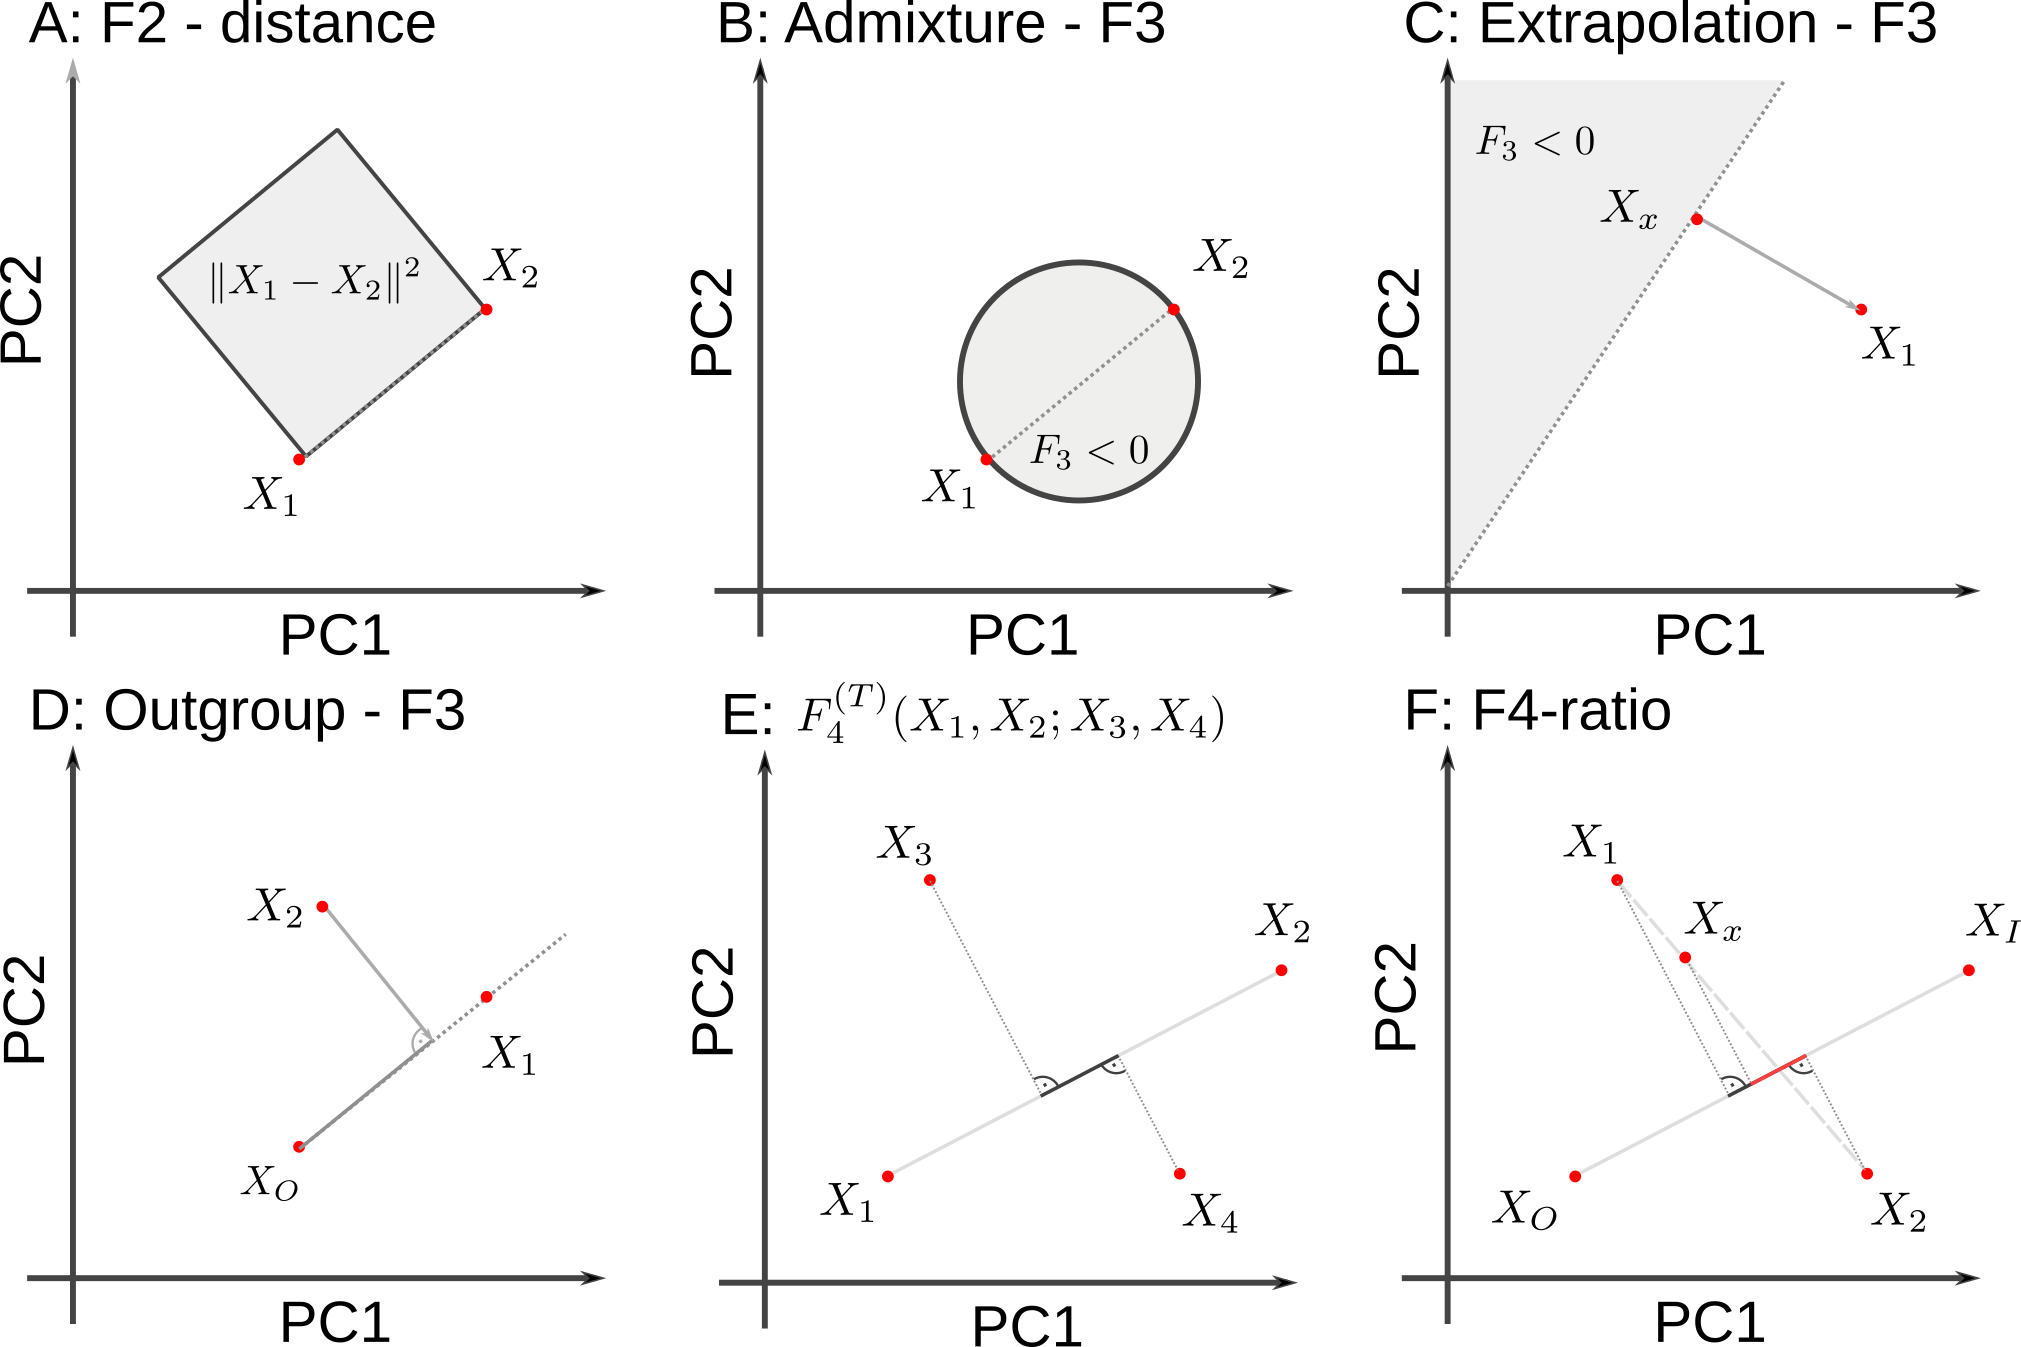
\includegraphics[width=\textwidth]{dummy_pca.png}
	\caption{\textbf{Geometric representation of $F$-statistics on 2D-PCA-plot.} A: $F_2$ represents the squared Euclidean distance between two points in PC-space. B: Admixture-$F_3(X_x; X_1, X_2)$ is negative if $X_x$ lies in the circle specified by the diameter $X_2-X_1$}. C: $F_3(X_x; X_1, X_2)$ is negative given $X_1, X_x$ if $X_2$ is in the gray space.  D: Outgroup-$F_3$ reflects the projection of $X_2 - X_O$ on $X_1 - X_O$. E: $F_4$ is the projection of $X_3 - X_4$ on $X_1-X_2$. F: If $X_x$ is admixed between $X_1$ and $X_2$, the admixture proportions will be projected.
\end{figure}

\subsubsection{$F_4$ and right angles}
The inner-product-interpretation of $F_4$ is similar to that of $F_3$, with the change that the two vectors we consider do not involve the same population. However, a finding of $F_4(X_1, X_2; X_3, X_4) = \langle X_1 - X_2, X_3 - X4 \rangle = 0$ similarly implies that the two vectors are orthogonal, and a non-zero value reflects the projection of one vector on the other.

\subsubsection{$F_4$-ratio}
\begin{eqnarray}
\frac{F_4(X_I, X_O; X_X, X_1)}{F_4(X_I, X_O; X_2, X_1)} &=& \frac{\norm{X_I-X_O}\norm{X_X-X_1}\cos(\alpha)}{\norm{X_I-X_O}\norm{X_2-X_1}\cos(\beta)}\nonumber\\
&=&\frac{\norm{X_X-X_1}\cos(\alpha)}{\norm{X_2-X_1}\cos(\beta)}\nonumber\\
&=& \frac{\norm{X_X' - X_1'}}{\norm{X_2' - X_1'}}
\end{eqnarray}
where $\alpha$ and $\beta$ are the angles between vectors, and $X_i'$ is the projection of $X_i$ on $X_I-X_O$.

Conjecture: Thus, we are measuring the distances between the admixing populations on the projected on the axis between $X_I$ and $X_O$. This ought to be valid only if $\langle X_1 - X_1', X_2 - X_2' \rangle$ are orthogonal to each other, and to $X_OX_I$, i.e.
$F_4(X_1, X_1', X_2, X_2') = 0$
 
	
\subsection{spectral analysis of admixture statistics}
\begin{enumerate}
	\item split F-stats by PCA basis vector
	\item same F-stat value may arise with different contribution from different PCs, should hint at distinct admixture events
	\item can use clustering to infer shared history?
	\item decomposition of admixture-F3?
%	\item rank of PCA vs qpAdm
\end{enumerate}

\section{Trees and admixture graphs in PCA-space}
\subsection{Trees}
Evolutionary trees are fundamental in phylogenetic analyses, as they, on a large, scale, approximate how taxa diversify. Within a species, applying trees is also very common, but more problematic as populations frequently do not evolve as discrete lineages; instead, they admix and diversify as much more continuous processes. This is largely due to the time-scales involved, speciation events that give rise to trees might often be similarly messy, but from a distance of millions of years these issues might disappear. 

Thus, when estimating trees from population genetic data, we must be very careful about whether the data is actually consistent with a tree, or belongs to some wider class of model.


Trees can be thought of as a collection of orthogonal dimensions; as drift on each branch is independent from every other branch. Thus, each sample is only 
\begin{enumerate}
	\item Trees
	\item Admixture Graphs
	\item Treelets
	\item simple trees, admixture graph
\end{enumerate}




\section{other orthogonal bases}
The most general ``model''-space for (centered) SNP-data $\MY$ is $\mathbb{R}^k$, where we allow each SNP to be in its own dimension, and treat all dimensions as independent. However, since in most analyses the number of samples $n \ll k$, we can place all SNPs in a $n$-dimensional subspace $\mathbb{R}^n$. (Could be restricted further to $[0,1]^k$, but that does not appear to add much).
If the data were normally distributed, $\MK$ has a $n$-dimensional Wishart-distribution with $k$ degrees of freedom. Since SNP are neither normal nor independent, the degrees of freedom might be considerably lower but we might still end up with something normally distributed.






	
\section{Technical considerations}
	\subsection{SNP weighting}
	It is clear that weighting SNP will have some effect on the resulting PCAs. Upweighting rare variants e.g. will emphasis recent events, as rare variance in the sample are more likely to be recent.
	
	
	\subsection{Missing data}
	
	\subsection{What is a dimension?}
	A single population at a particular point in time can be thought of as a single point in allele-frequency space, given by it's $p$-dimensional locus of allele frequencies in that population. If this population evolves for some time in isolation, allele frequencies will change due to genetic drift; i.e. the population evolves along a single tree branch in the interpretation of \cite{patterson2012}. If we now add a second population, it will behave exactly the same, and the drift in the second population will be uncorrelated to the first, i.e. it evolves in a second dimension. Thus, if we have two populations that descend from the same ancestral population in isolation, they can be thought of as evolving along orthognal dimensions from the same point. This argument is at the foundation of F-statistics.
	
	
	\section{outtakes}
	PCA from $\MX$
	\begin{equation}
	\MK = \MY \MY^T = \MC\MX\MX^T \MC = \MP\MP^T
	\end{equation}
	

\bibliography{main}
\end{document}